\paragraph{Thực nghiệm với Beijing Air Quality} \hfill \\
Đây là bài toán dự báo đa biến (Multivariate Time Series Forecasting). Mục tiêu là dự báo nồng độ bụi mịn PM2.5 dựa trên các yếu tố lịch sử và khí tượng như nhiệt độ, áp suất, tốc độ gió.

\paragraph{Mô hình Multivariate LSTM} \hfill \\
Mô hình sử dụng cơ chế cửa sổ trượt (sliding window) với độ dài 24 giờ (\textbf{LOOK\_BACK = 24}) để dự báo giá trị cho giờ tiếp theo. Tổng số tham số là \textbf{121,665}.

\paragraph{Kết quả thực nghiệm} \hfill \\
Mô hình đạt độ chính xác cực cao với \textbf{R² score là 0.9457}. Chỉ số \textbf{Test RMSE là 21.1601 µg/m³}.

\begin{figure}[H]
    \centering
    \begin{minipage}{0.48\textwidth}
        \centering
        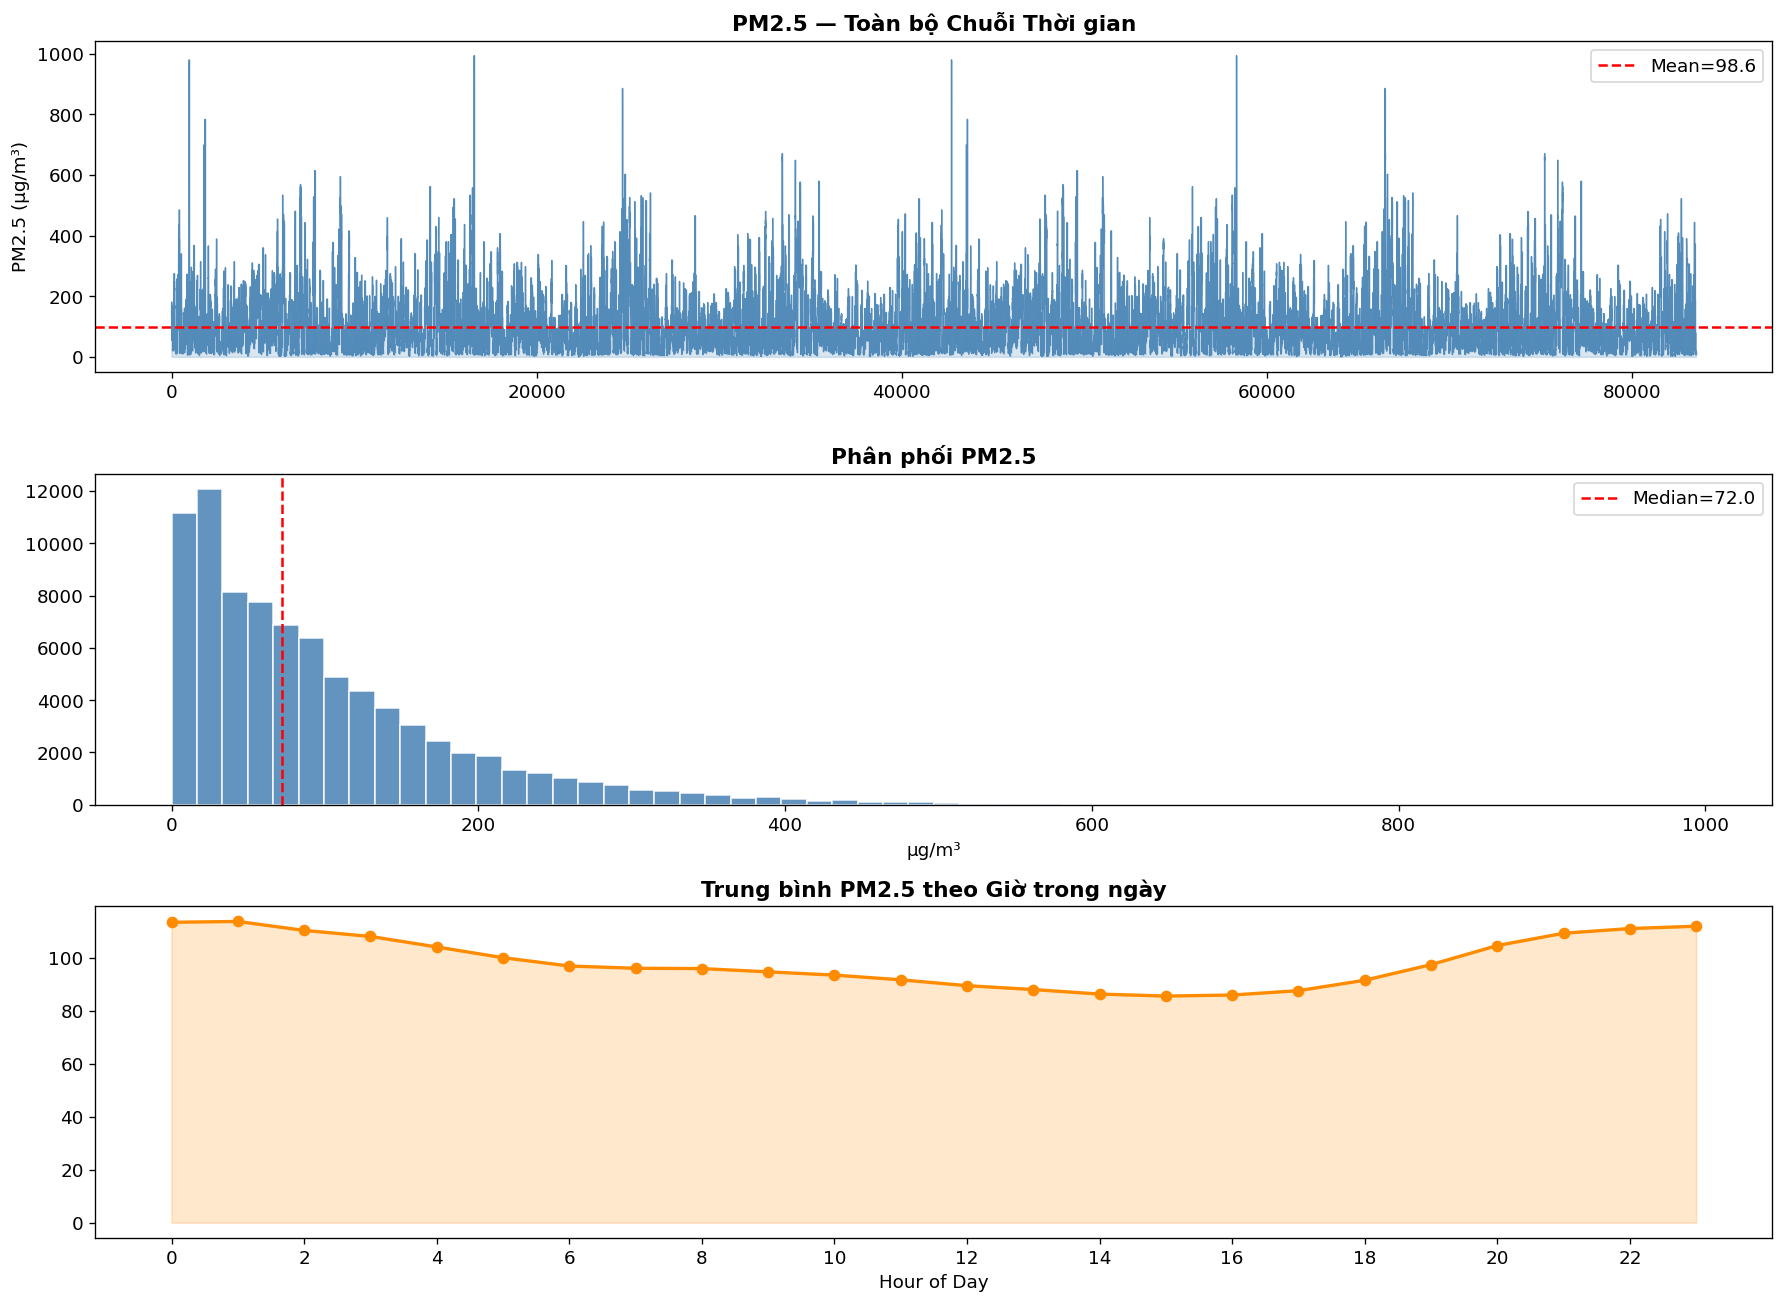
\includegraphics[width=\linewidth]{Chương_4/results/beijing_air_quality/01_time_series_eda.png}
        \caption{Biến thiên nồng độ PM2.5 theo thời gian}
        \label{fig:air_eda}
    \end{minipage}
    \hfill
    \begin{minipage}{0.48\textwidth}
        \centering
        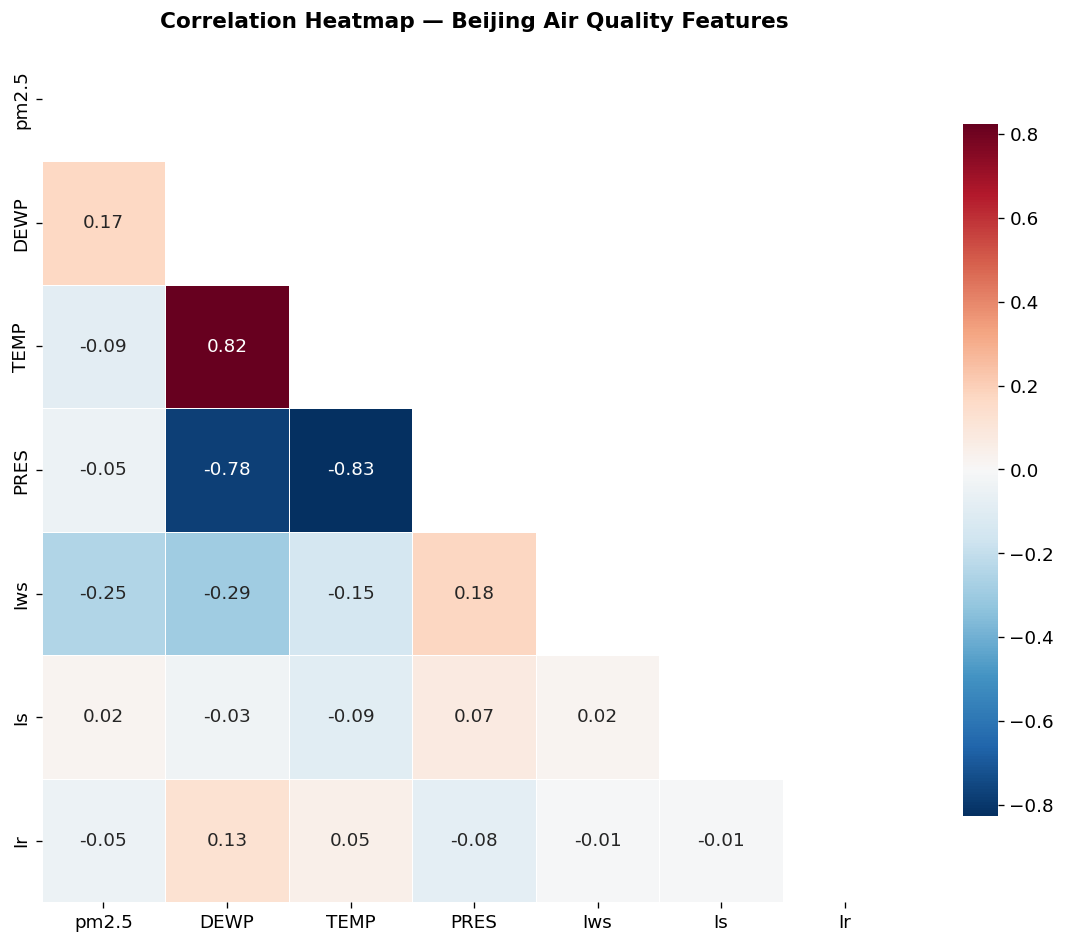
\includegraphics[width=\linewidth]{Chương_4/results/beijing_air_quality/02_correlation_heatmap.png}
        \caption{Tương quan giữa các yếu tố khí tượng}
        \label{fig:air_corr}
    \end{minipage}
\end{figure}

\begin{figure}[H]
    \centering
    \begin{minipage}{0.31\textwidth}
        \centering
        
\includegraphics[width=\linewidth]{Chương_4/results/beijing_air_quality/03_training_history.png}
        \caption{Lịch sử huấn luyện}
        \label{fig:air_history}
    \end{minipage}
    \hfill
    \begin{minipage}{0.31\textwidth}
        \centering
        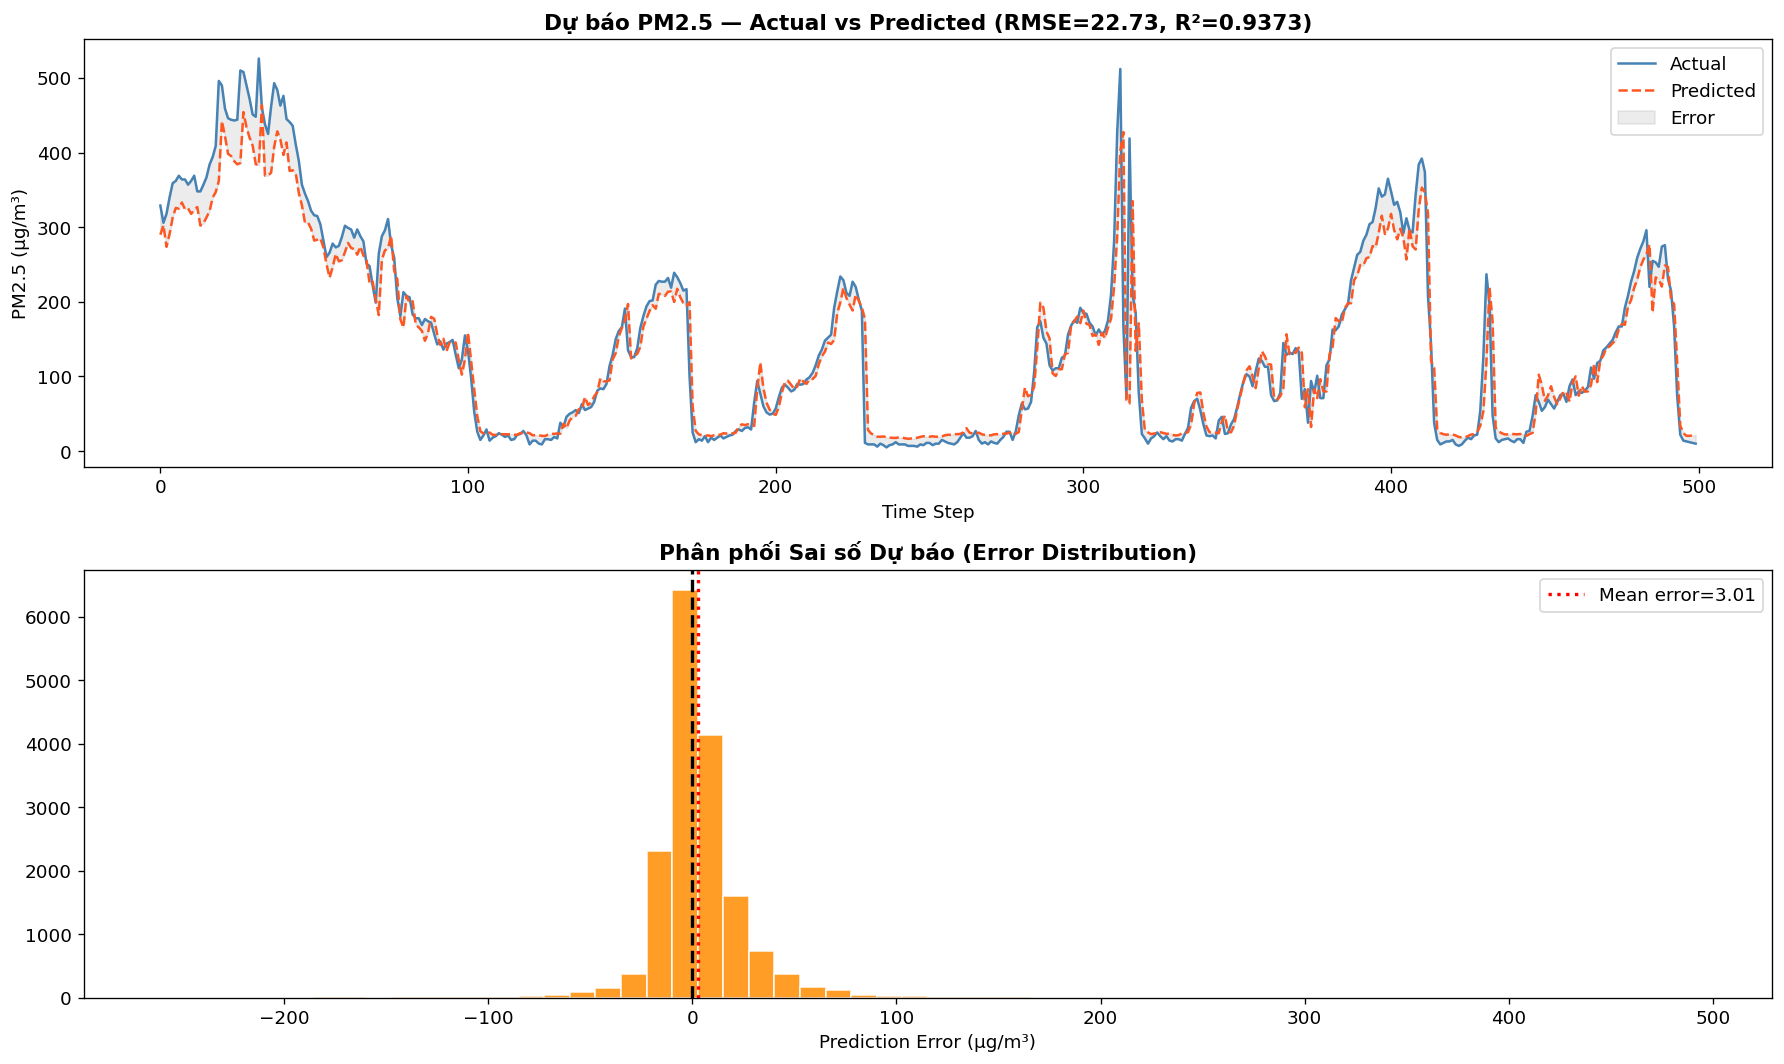
\includegraphics[width=\linewidth]{Chương_4/results/beijing_air_quality/04_forecast_vs_actual.png}
        \caption{Dự báo vs Thực tế}
        \label{fig:air_forecast}
    \end{minipage}
    \hfill
    \begin{minipage}{0.31\textwidth}
        \centering
        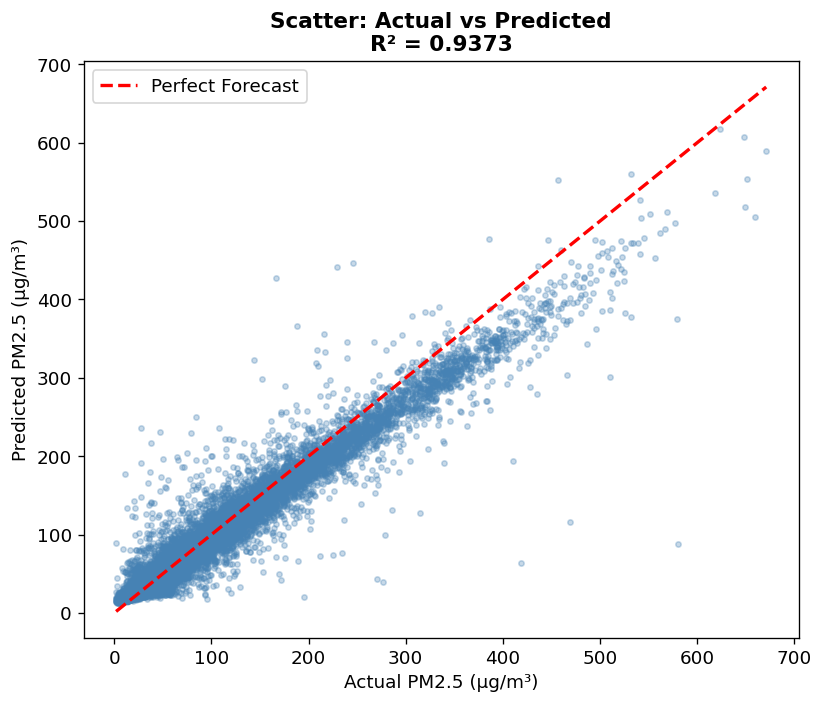
\includegraphics[width=\linewidth]{Chương_4/results/beijing_air_quality/05_scatter_actual_vs_pred.png}
        \caption{Actual vs Predicted}
        \label{fig:air_scatter}
    \end{minipage}
\end{figure}


\paragraph{Phụ lục: Quy trình thực nghiệm chi tiết} \hfill \\
Dưới đây là các bước triển khai chi tiết trên môi trường Jupyter Notebook:

\begin{figure}[H]
    \centering
    
\includegraphics[width=0.9\linewidth]{Chương_4/docs/ch4/1.png}
    \caption{Tải dữ liệu: Đọc file CSV chứa các chỉ số chất lượng không khí tại Bắc Kinh từ 2010-2014.}
\end{figure}

\begin{figure}[H]
    \centering
    
\includegraphics[width=0.9\linewidth]{Chương_4/docs/ch4/2.png}
    \caption{Kiểm tra dữ liệu thiếu: Xác định nồng độ PM2.5 bị thiếu tại một số thời điểm (NaN).}
\end{figure}

\begin{figure}[H]
    \centering
    
\includegraphics[width=0.9\linewidth]{Chương_4/docs/ch4/3.png}
    \caption{Xử lý giá trị thiếu: Sử dụng phương pháp nội suy tuyến tính (Interpolation) để lấp đầy các khoảng trống dữ liệu.}
\end{figure}

\begin{figure}[H]
    \centering
    
\includegraphics[width=0.9\linewidth]{Chương_4/docs/ch4/4.png}
    \caption{EDA chuỗi thời gian: Trực quan hóa biến động PM2.5 qua các năm để thấy rõ tính mùa vụ và xu hướng.}
\end{figure}

\begin{figure}[H]
    \centering
    
\includegraphics[width=0.9\linewidth]{Chương_4/docs/ch4/5.png}
    \caption{Trích xuất đặc trưng thời gian: Chuyển đổi các cột Year, Month, Day thành các đặc trưng số học hỗ trợ mô hình.}
\end{figure}

\begin{figure}[H]
    \centering
    
\includegraphics[width=0.9\linewidth]{Chương_4/docs/ch4/6.png}
    \caption{Chuẩn hóa dữ liệu: Sử dụng MinMaxScaler để đưa các biến khí tượng về khoảng [0, 1] nhằm tối ưu hóa hội tụ.}
\end{figure}

\begin{figure}[H]
    \centering
    
\includegraphics[width=0.9\linewidth]{Chương_4/docs/ch4/7.png}
    \caption{Chuyển đổi sang học có giám sát: Tạo cấu trúc cửa sổ trượt (sliding window) với `LOOK\_BACK = 24` giờ.}
\end{figure}

\begin{figure}[H]
    \centering
    
\includegraphics[width=0.9\linewidth]{Chương_4/docs/ch4/8.png}
    \caption{Phân tách dữ liệu: Chia tập Train/Test theo trình tự thời gian để đảm bảo tính thực tế của dự báo.}
\end{figure}

\begin{figure}[H]
    \centering
    
\includegraphics[width=0.9\linewidth]{Chương_4/docs/ch4/9.png}
    \caption{Kiến trúc Multivariate LSTM: Định nghĩa mô hình với các lớp LSTM và Dense để xử lý dữ liệu đa biến.}
\end{figure}

\begin{figure}[H]
    \centering
    
\includegraphics[width=0.9\linewidth]{Chương_4/docs/ch4/10.png}
    \caption{Nhật ký huấn luyện: Theo dõi quá trình giảm hàm mất mát (Loss) qua từng Epoch trên cả hai tập dữ liệu.}
\end{figure}

\begin{figure}[H]
    \centering
    
\includegraphics[width=0.9\linewidth]{Chương_4/docs/ch4/11.png}
    \caption{Lịch sử hội tụ: Đồ thị MSE và MAE khẳng định mô hình học ổn định và hội tụ nhanh chóng.}
\end{figure}

\begin{figure}[H]
    \centering
    
\includegraphics[width=0.9\linewidth]{Chương_4/docs/ch4/12.png}
    \caption{Mã nguồn đánh giá: Triển khai các hàm vẽ biểu đồ so sánh Dự báo vs Thực tế và phân tích sai số.}
\end{figure}

\begin{figure}[H]
    \centering
    
\includegraphics[width=0.9\linewidth]{Chương_4/docs/ch4/13.png}
    \caption{Kết quả dự báo chi tiết: Đồ thị đường bám sát giá trị thực tế và biểu đồ phân phối sai số tập trung quanh mức 0.}
\end{figure}

\begin{figure}[H]
    \centering
    
\includegraphics[width=0.9\linewidth]{Chương_4/docs/ch4/14.png}
    \caption{Biểu đồ phân tán (Scatter Plot): Sự tương quan chặt chẽ giữa giá trị thực tế và dự đoán ($R^2 = 0.9457$).}
\end{figure}
